\chapter{Metodologia}\label{cap:metodologia}

Este capítulo descreve a abordagem adotada para investigar a aplicabilidade da coerência
\textit{Wavelet} alternativa de \citeonline{schuck2019} como ferramenta de caracterização
dos padrões de escoamento bifásico no arranjo experimental do LETEF.
Em vez de utilizar os sinais dos sensores no domínio do tempo, o método construiu, para
cada ensaio, um sinal unidimensional de brilho no domínio \textit{espacial}, obtido a
partir de um panorama reconstruído das imagens da câmera de alta velocidade, e aplicou a
formulação de \citeonline{schuck2019} a pares desses sinais.
A \autoref{sec:met-visao} apresenta uma visão geral do método; as seções seguintes
descrevem os dados, o pré-processamento, o cálculo da coerência e a análise das
assinaturas espectrais, comparando os campos WPS, WCS e WCO entre ensaios de um mesmo
padrão (repetibilidade intra-padrão) e entre padrões distintos (separação inter-padrão).

% =========================================================
\section{Visão geral do método proposto}\label{sec:met-visao}
% =========================================================

A abordagem consiste em calcular a coerência \textit{Wavelet} alternativa
$\widetilde{\gamma}_{xy}(a)$ entre dois sinais espaciais de brilho $x$ e $y$, cada um
extraído do panorama reconstruído de um ensaio, e verificar se as assinaturas espectrais
resultantes são reprodutíveis dentro de um mesmo padrão de escoamento e distinguíveis
entre padrões distintos. Os dois sinais comparados são \textit{dois ensaios} (\textit{runs}):
no modo intra-padrão, dois ensaios do mesmo padrão, para avaliar a repetibilidade; no modo
inter-padrão, ensaios de padrões diferentes, para avaliar a separação. A hipótese investigada
é se a estrutura espectral do acoplamento, expressa por $\widetilde{\gamma}_{xy}(a)$ em
função da escala, se mantém consistente entre ensaios de um mesmo padrão e varia
sistematicamente de um padrão para outro, refletindo a dinâmica distinta da interface
líquido-vapor em cada regime. A coerência $\widetilde{\gamma}_{xy}(a)$ é o descritor
principal; o perfil de potência média $|\text{WPS}|$ por comprimento de onda complementa
a análise.

O \textit{pipeline} é composto pelas seguintes etapas:

\begin{enumerate}
  \item construção do sinal espacial de brilho a partir do panorama de cada ensaio;
  \item pré-processamento dos sinais;
  \item cálculo da autocorrelação de cada ensaio e da correlação cruzada entre os dois
        ensaios;
  \item aplicação da CWT nas funções de correlação e obtenção de
        $\widetilde{P}_x(a)$, $\widetilde{P}_y(a)$, $\widetilde{C}_{xy}(a)$ e da coerência
        alternativa $\widetilde{\gamma}_{xy}(a)$ no atraso nulo;
  \item análise das assinaturas espectrais (campos WCO e WCS e perfil de potência média)
        por padrão de escoamento, nos modos intra-padrão e inter-padrão.
\end{enumerate}

A \autoref{fig:pipeline} resume esquematicamente o fluxo de processamento.

\begin{figure}[htb]
  \centering
  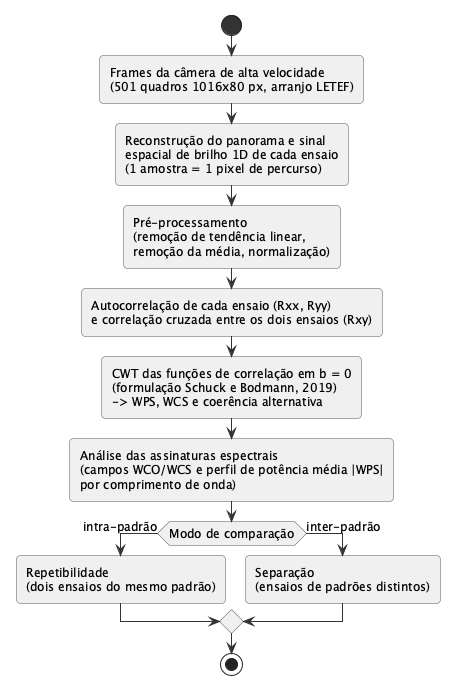
\includegraphics[width=0.55\textwidth]{figuras/pipeline-wco}
  \caption{Fluxograma do método para caracterização dos padrões de escoamento
           por coerência \textit{Wavelet} alternativa a partir de sinais espaciais de brilho.}
  \label{fig:pipeline}
  \fonte{Elaborado pelo autor.}
\end{figure}

% =========================================================
\section{Dados experimentais}\label{sec:met-dados}
% =========================================================

Os dados utilizados neste trabalho são os quadros (\textit{frames}) da câmera de alta
velocidade registrados por \citeonline{deoliveira2021} no arranjo experimental do LETEF,
descrito na \autoref{sec:arranjo}. O fluido estudado é o isobutano (R600a), a
27\textdegree{}C de temperatura de saturação. Cada ensaio corresponde a uma sequência de
501 quadros de $1016 \times 80$ pixels, registrados na seção de visualização para uma
combinação específica de fluxo mássico $G$ e fluxo de calor $q''$, abrangendo as seis
condições de padrão de escoamento identificadas naquele trabalho: bolha dispersa,
\textit{plug}, \textit{slug}, \textit{churn}, anular ondulado e anular liso.

A partir de cada sequência de quadros, reconstruiu-se um panorama do escoamento. Para cada
par de quadros consecutivos mediu-se o deslocamento horizontal do escoamento por correlação
cruzada dos perfis de brilho médios da banda central do tubo; costurou-se, então, uma tira
central de cada quadro na posição medida, formando uma imagem panorâmica cuja largura é o
deslocamento acumulado ao longo do ensaio. O panorama bidimensional foi colapsado em um
sinal unidimensional pela média das colunas, em duas variantes: a média das linhas 20 a 59
(núcleo do escoamento, denominada \textit{cropped}) e a linha central 40 (\textit{center}).
No sinal resultante, uma amostra corresponde a um pixel de percurso do escoamento no tubo:
trata-se, portanto, de um sinal puramente \textit{espacial}, sem eixo de tempo nem
frequência de amostragem associada.

A escolha do domínio espacial em vez do domínio do tempo decorre do número de amostras
disponível. No domínio do tempo, cada ensaio dispõe de apenas 501 quadros; a série temporal
efetivamente reamostrada usada como contraparte neste trabalho reduz-se a cerca de 287
amostras. Já o panorama espacial reconstruído contém, conforme o ensaio, de algumas centenas
a mais de vinte mil pixels de percurso, situando-se tipicamente na faixa de milhares de
amostras (por exemplo, os ensaios de \textit{churn} analisados têm entre 7\,584 e 9\,586
pixels). O sinal espacial oferece, assim, uma ou duas ordens de grandeza mais amostras do
que a série temporal, o que se traduz em maior resolução espectral e na ausência de um teto
de Nyquist atrelado à taxa de quadros da câmera, condição vantajosa para a estimativa das
funções de correlação exigidas pela formulação de \citeonline{schuck2019}.

Para cada ensaio, o padrão de escoamento foi previamente identificado por análise visual
das imagens da câmera de alta velocidade na seção de visualização, conforme descrito por
\citeonline{deoliveira2021}. Essa identificação prévia constitui o rótulo de referência
utilizado para avaliar se as assinaturas de coerência \textit{Wavelet} correspondem a cada
padrão. Entre os padrões, apenas o \textit{churn} ($n = 10$) e o anular ondulado ($n = 9$)
dispõem de ensaios suficientes para sustentar a análise de repetibilidade intra-padrão; os
demais (\textit{plug}, \textit{slug} e \textit{slug}--\textit{churn}) têm $n \leq 4$ e são
tratados de forma ilustrativa.

A comparação foi feita em dois modos, ambos restritos aos cinco padrões com pelo menos dois
ensaios (\textit{churn}, com dez ensaios; anular ondulado, com nove; \textit{plug}, com quatro;
\textit{slug}, com três; e \textit{slug}--\textit{churn}, com dois), que somam vinte e oito
ensaios. Os padrões com um único ensaio (bolha dispersa, anular liso e \textit{plug}--\textit{slug})
ficaram de fora por não formarem pares. No modo intra-padrão, avaliaram-se todas
as combinações de dois ensaios de um mesmo padrão, o que dá noventa e um pares (quarenta e cinco
de \textit{churn}, trinta e seis de anular ondulado, seis de \textit{plug}, três de \textit{slug}
e um de \textit{slug}--\textit{churn}). No modo inter-padrão, formaram-se os pares de ensaios de
padrões distintos, ou seja, o produto cartesiano dos ensaios de cada par de padrões, chegando-se
a duzentos e oitenta e sete pares de ensaios repartidos pelas dez combinações possíveis dos cinco
padrões. A ordem dentro de cada par define apenas qual ensaio entra como primeiro sinal
(prioridade \textit{churn}, anular ondulado e, para os demais, ordem alfabética); como a coerência
é definida por escala, essa ordem não altera seu valor. Ambos os modos empregam o cálculo de
coerência \textit{Wavelet} alternativa descrito nas seções seguintes, diferindo apenas na regra de
emparelhamento dos ensaios.

% =========================================================
\section{Pré-processamento dos sinais}\label{sec:met-preproc}
% =========================================================

Antes de calcular as funções de correlação, cada sinal espacial passou pelas seguintes
etapas de pré-processamento:

\begin{enumerate}
  \item Remoção de tendência: subtração de uma tendência linear ajustada ao sinal, para
        eliminar derivas de baixa frequência introduzidas por variações lentas de
        iluminação e pela costura do panorama, que não carregam informação sobre a
        morfologia do escoamento;
  \item Remoção da média: subtração do valor médio, eliminando a componente contínua e
        garantindo que a autocorrelação seja bem definida;
  \item Normalização: divisão pelo desvio padrão amostral, garantindo variância unitária
        e tornando as funções de correlação comparáveis entre ensaios com diferentes
        condições operacionais. A formulação de \citeonline{schuck2019} pressupõe que os
        sinais sejam realizações de processos estacionários, hipótese sob a qual as funções
        de auto e correlação cruzada estão bem definidas.
\end{enumerate}

A formulação alternativa de \citeonline{schuck2019} pressupõe processos estacionários.
No domínio espacial, essa hipótese equivale à homogeneidade estatística do panorama ao
longo do eixo de percurso: como cada ensaio de \citeonline{deoliveira2021} foi coletado com
$G$ e $q''$ fixos, em regime estabelecido, o padrão de escoamento mantém-se estatisticamente
uniforme ao longo do trecho reconstruído, conforme o protocolo experimental descrito na
\autoref{sec:arranjo}.

% =========================================================
\section{Cálculo da coerência \textit{Wavelet} alternativa}\label{sec:met-wco}
% =========================================================

O cálculo da coerência \textit{Wavelet} alternativa seguiu a formulação de
\citeonline{schuck2019}, conforme descrita na \autoref{sec:wps-wcs-wco}. As etapas foram
as seguintes:

\begin{enumerate}
  \item Autocorrelação e correlação cruzada: calcularam-se numericamente a autocorrelação
        do primeiro ensaio $R_{xx}(\tau)$, a autocorrelação do segundo ensaio
        $R_{yy}(\tau)$ e a correlação cruzada entre os dois ensaios $R_{xy}(\tau)$ a partir
        dos sinais espaciais pré-processados, para defasagens $\tau$ de $-(N-1)$ a $N-1$
        pixels, em que $N$ é o comprimento do sinal (variável de um ensaio para outro, da
        ordem de milhares de pixels), com normalização enviesada, dividindo cada soma por
        $N$;
  \item CWT das funções de correlação: aplicou-se a CWT de \textit{Wavelet} de Morlet
        complexa a cada função de correlação, avaliada em $b = 0$, sobre uma grade
        logarítmica de 200 escalas cobrindo comprimentos de onda de 50 a 3\,000 pixels,
        faixa escolhida para englobar as estruturas espaciais características dos padrões
        de escoamento. A realização concreta empregou a \textit{Wavelet} \texttt{cmor2.0-0.9549}
        da biblioteca \textit{PyWavelets} (largura de banda 2,0 e frequência central
        0,9549), conforme detalhado na \autoref{sec:met-wco-morlet};
  \item Espectros alternativos: calcularam-se o espectro de potência alternativo do
        primeiro ensaio $\widetilde{P}_x(a) = |W_{R_{xx}}(a,0)|$, o do segundo ensaio
        $\widetilde{P}_y(a) = |W_{R_{yy}}(a,0)|$ e o espectro cruzado alternativo
        $\widetilde{C}_{xy}(a) = |W_{R_{xy}}(a,0)|$, conforme as \autoref{eq:wps-alt} e
        \autoref{eq:wcs-alt};
  \item Coerência por escala: obteve-se a coerência \textit{Wavelet} alternativa
        $\widetilde{\gamma}_{xy}(a) = \widetilde{C}_{xy}(a)^2\,/\,[\widetilde{P}_x(a)\cdot\widetilde{P}_y(a)]$
        (\autoref{eq:wco-alt}), avaliada no atraso nulo, resultando em uma curva de
        coerência em função do comprimento de onda de cada escala.
\end{enumerate}

A implementação foi realizada em Python, com as bibliotecas \textit{NumPy} e \textit{SciPy}
para os cálculos de correlação e \textit{PyWavelets} (\textit{pywt}) para a CWT. Antes da
aplicação aos dados reais, a implementação foi validada com sinais sintéticos de frequência,
fase e razão sinal-ruído controladas, seguindo o procedimento descrito por
\citeonline{schuck2019}, para confirmar que as equações estão corretamente implementadas e
que o método recupera os resultados esperados.

\subsection{Parametrização da \textit{Wavelet} de Morlet}\label{sec:met-wco-morlet}

A moldura teórica da \autoref{sec:cwt} descreve a \textit{Wavelet} de Morlet complexa pela
frequência central adimensional $\omega_0 = 6$. A implementação usou a \textit{Wavelet}
complexa de Morlet \texttt{cmor2.0-0.9549} do \textit{PyWavelets}, cujos parâmetros de
largura de banda (2,0) e de frequência central (0,9549) definem a realização discreta
concreta dessa família. A conversão entre escala $a$ e comprimento de onda $\lambda$ segue
a frequência central da \textit{Wavelet}, obtida por \texttt{pywt.central\_frequency}, de
modo que cada escala da grade corresponde a um comprimento de onda em pixels. Todas as
grandezas espectrais deste capítulo são, portanto, expressas em comprimento de onda (pixels),
e não em frequência temporal.

% =========================================================
\section{Análise das assinaturas espectrais}\label{sec:met-analise}
% =========================================================

Para cada padrão de escoamento, os campos de coerência $\widetilde{\gamma}_{xy}(a)$ e de
espectro cruzado $\widetilde{C}_{xy}(a)$ de pares de ensaios foram comparados entre si,
permitindo avaliar visualmente a consistência intra-padrão e a separação inter-padrão. A
coerência alternativa é o descritor principal da análise. Como leitura complementar,
extraiu-se de cada ensaio o perfil de potência média $|\text{WPS}|$ em função do comprimento
de onda, isto é, a média do módulo dos coeficientes da CWT da autocorrelação ao longo dos
atrasos, que resume em uma curva os comprimentos de onda em que a energia espectral do
ensaio se concentra:

\begin{enumerate}
  \item Comprimento de onda dominante: escala $a^*$ em que o perfil de potência média
        $|\text{WPS}|$ é máximo, indicando o comprimento de onda característico das
        estruturas espaciais do padrão analisado;
  \item Coerência máxima: valor de pico $\widetilde{\gamma}_{xy}(a^*)$, como indicador da
        similaridade da estrutura espectral entre os dois ensaios comparados.
\end{enumerate}

Esta análise tem caráter exploratório: não se define limiar de separabilidade a priori.
A avaliação é qualitativa, baseada na consistência dos campos $\widetilde{\gamma}_{xy}(a)$
e dos perfis de potência média entre ensaios de um mesmo padrão (repetibilidade
intra-padrão) e na distinção desses campos entre padrões diferentes (separação
inter-padrão), com o objetivo de determinar se a coerência \textit{Wavelet} alternativa
constitui um descritor viável para a caracterização dos padrões de escoamento. A repetibilidade
intra-padrão foi verificada sobre os noventa e um pares de ensaios de mesmo padrão, e a separação
inter-padrão sobre os duzentos e oitenta e sete pares de ensaios de padrões distintos.

% =========================================================
\section{Aplicação passo a passo das equações: ensaio de \textit{churn}}\label{sec:met-exemplo}
% =========================================================

Para tornar concreto o encadeamento das equações, esta seção percorre as cinco etapas do
\textit{pipeline} aplicadas a dois ensaios de \textit{churn}.

% ---------------------------------------------------------
\subsection{Entrada}\label{sec:met-exemplo-entrada}
% ---------------------------------------------------------

Os sinais espaciais $x[n]$ e $y[n]$ correspondem a dois ensaios distintos classificados
como \textit{churn}, extraídos da variante \textit{cropped} do panorama (média das linhas
20 a 59). Os dois ensaios têm 9\,586 e 8\,829 pixels de percurso; como o cálculo emparelha
os sinais pelo menor comprimento, adotou-se $N = 8\,829$ amostras espaciais, com passo de
1 pixel. Após a remoção de tendência, da média e a normalização pelo desvio padrão
(\autoref{sec:met-preproc}), tem-se $\bar{x} = \bar{y} = 0$ e $\sigma_x = \sigma_y = 1$.

% ---------------------------------------------------------
\subsection{Passo~1 — Autocorrelação e correlação cruzada}\label{sec:met-exemplo-p1}
% ---------------------------------------------------------

A versão discreta da \autoref{eq:autocorr} é a função de autocorrelação $R_{xx}[m]$
do primeiro ensaio, com normalização enviesada:

\begin{equation}\label{eq:autocorr-disc}
  R_{xx}[m] = \frac{1}{N}\sum_{n=0}^{N-1-|m|} x[n]\,x[n+m],
  \qquad m = -(N{-}1), \ldots, N{-}1.
\end{equation}

\noindent
A função de correlação cruzada $R_{xy}[m]$ entre os dois ensaios é discretizada de forma
análoga a partir da \autoref{eq:crosscorr}:

\begin{equation}\label{eq:crosscorr-disc}
  R_{xy}[m] = \frac{1}{N}\sum_{n=0}^{N-1-|m|} x[n]\,y[n+m],
  \qquad m = -(N{-}1), \ldots, N{-}1.
\end{equation}

\noindent
O atraso $m$ é medido em pixels. Um eventual pico de $R_{xy}[m]$ em $m^* \neq 0$ reflete um
deslocamento de fase espacial entre os dois ensaios, e não uma relação de causa e efeito:
por serem realizações turbulentas independentes do mesmo padrão, os dois sinais não
compartilham uma fase espacial comum, de modo que a informação relevante está na estrutura
espectral das funções de correlação, não na posição do pico.

% ---------------------------------------------------------
\subsection{Passo~2 — CWT das funções de correlação}\label{sec:met-exemplo-p2}
% ---------------------------------------------------------

A CWT de \textit{Wavelet} de Morlet complexa (\autoref{sec:cwt}; realização
\texttt{cmor2.0-0.9549}, conforme \autoref{sec:met-wco-morlet}) é aplicada às funções de
autocorrelação do primeiro ensaio $R_{xx}[\tau]$, de autocorrelação do segundo ensaio
$R_{yy}[\tau]$ e de correlação cruzada entre os dois $R_{xy}[\tau]$, avaliadas em $b = 0$
(atraso nulo do domínio da transformada, que corresponde ao ponto de referência
das funções de correlação). Para uma escala $a_k$, o coeficiente é:

\begin{equation}\label{eq:cwt-disc}
  W_{R_{xx}}(a_k,\, 0) = \frac{\delta\tau}{\sqrt{a_k}}
  \sum_{m=-(N{-}1)}^{N{-}1}
  R_{xx}[m]\,\psi^*\!\!\left(\frac{-m\,\delta\tau}{a_k}\right),
\end{equation}

\noindent
em que $\delta\tau = 1\,\text{px}$ é o passo espacial e
$\psi(u)$ é a \textit{Wavelet} de Morlet complexa (\autoref{sec:cwt}). A operação é
aplicada às três funções de correlação, produzindo, para cada escala $a_k$ da grade, os
coeficientes da CWT: $W_{R_{xx}}(a_k,0)$, $W_{R_{yy}}(a_k,0)$ e $W_{R_{xy}}(a_k,0)$. Cada
escala $a_k$ corresponde a um comprimento de onda $\lambda_k$ em pixels, obtido pela
frequência central da \textit{Wavelet} (\autoref{sec:met-wco-morlet}). A amplitude dos
coeficientes reflete a atividade das funções de correlação em cada comprimento de onda,
realçando as escalas associadas às estruturas espaciais do \textit{churn}.

% ---------------------------------------------------------
\subsection{Passo~3 — Espectros alternativos}\label{sec:met-exemplo-p3}
% ---------------------------------------------------------

Aplicando as \autoref{eq:wps-alt} e \autoref{eq:wcs-alt} aos coeficientes do
\autoref{sec:met-exemplo-p2}, obtêm-se: o espectro de potência alternativo do primeiro
ensaio, $\widetilde{P}_x(a_k)$; o do segundo ensaio, $\widetilde{P}_y(a_k)$; e o espectro
cruzado alternativo entre os dois, $\widetilde{C}_{xy}(a_k)$, uma tripla de valores reais
não negativos para cada escala $a_k$. Os espectros $\widetilde{P}_x$ e $\widetilde{P}_y$
descrevem a distribuição de energia de cada ensaio por comprimento de onda, enquanto
$\widetilde{C}_{xy}$ quantifica a energia conjunta dos dois sinais em cada escala.

% ---------------------------------------------------------
\subsection{Passo~4 — Coerência alternativa}\label{sec:met-exemplo-p4}
% ---------------------------------------------------------

Aplicando a \autoref{eq:wco-alt} aos espectros do \autoref{sec:met-exemplo-p3},
obtém-se a coerência \textit{Wavelet} alternativa $\widetilde{\gamma}_{xy}(a)$,
uma curva com valores em $[0, 1]$ que expressa, para cada comprimento de onda $\lambda_k$,
o grau de similaridade da estrutura espectral entre os dois ensaios naquela escala, no
atraso nulo. O valor em cada escala indica o grau de acoplamento espectral entre os dois
ensaios naquele comprimento de onda, assumindo valor próximo da unidade quando as estruturas
espaciais se manifestam de forma consistente entre os ensaios. O procedimento é repetido para
todas as escalas da grade, produzindo a curva completa $\widetilde{\gamma}_{xy}(a)$.

% ---------------------------------------------------------
\subsection{Passo~5 — Extração das métricas espectrais}\label{sec:met-exemplo-p5}
% ---------------------------------------------------------

A partir da curva completa de coerência $\widetilde{\gamma}_{xy}(a)$ e do perfil de
potência média $|\text{WPS}|$, identificam-se:
(i)~o comprimento de onda dominante $\lambda^*$, isto é, a escala em que o perfil de
potência média é máximo, associado às estruturas espaciais do padrão descritas na
\autoref{sec:padroes}; e
(ii)~a coerência máxima $\widetilde{\gamma}_{xy}(a^*)$, como indicador da similaridade da
estrutura espectral entre os dois ensaios comparados.

Essas grandezas constituem a assinatura espectral do par de ensaios. Ao comparar os campos
de coerência e os perfis de potência de vários ensaios classificados como \textit{churn},
avalia-se a repetibilidade intra-padrão. Ao comparar ensaios de padrões diferentes, avalia-se
a separabilidade inter-padrão.
